\documentclass[12pt]{article}

\usepackage{fontspec}
\newfontfamily\handwriting{a-casual-handwritten-pen}[Path=../assets/fonts/,Extension=.ttf,Scale=1.5]
\newfontfamily\comic{Comic Neue}

\usepackage[utf8]{inputenc}
\usepackage{amsmath}
\usepackage{amssymb}
\usepackage{enumitem}
\usepackage{xcolor}
\usepackage{soul}
\usepackage{tikz}
\usepackage[most]{tcolorbox}
\usepackage{titlesec}
\usepackage{multicol}
\usepackage{environ}

\usetikzlibrary{fit, positioning, arrows.meta}

% --- Custom Colors ---
\definecolor{primaryblue}{RGB}{42, 111, 151}
\definecolor{exbg}{RGB}{255, 240, 245}
\definecolor{rulebg}{RGB}{232, 245, 233}
\definecolor{highlight}{RGB}{255, 243, 176}
\definecolor{pinkanno}{RGB}{255, 105, 180}
\definecolor{purpleanno}{RGB}{147, 112, 219}
\definecolor{solutionbg}{RGB}{245, 245, 255}

% --- Header Styling ---
\titleformat{\section}{\color{primaryblue}\normalfont\Large\bfseries}{\thesection}{1em}{}
\titleformat{\subsection}{\color{primaryblue}\normalfont\large\bfseries}{\thesubsection}{1em}{}

% --- Friendly Boxes ---
% --- Auto-numbered Example Box ---
\newcounter{examplenum}

\newtcolorbox{friendlyexbox}[1]{
    colback=exbg,
    colframe=pinkanno!50,
    arc=5pt,
    title=\textbf{#1},
    coltitle=black,
    attach title to upper,
    after title={:\quad}
}

\newenvironment{friendlyex}{%
    \refstepcounter{examplenum}%
    \begin{friendlyexbox}{Example \theexamplenum}%
}{%
    \end{friendlyexbox}%
}

\newtcolorbox{friendlyrule}[1]{
    colback=rulebg,
    colframe=primaryblue!30,
    arc=5pt,
    fonttitle=\bfseries,
    title={#1},
    coltitle=primaryblue
}

\newcommand{\funhl}[1]{\sethlcolor{highlight}\hl{#1}}

% --- Show/Hide Solutions ---
\newif\ifshowsolutions

% Uncomment the next line to show solutions.
\showsolutionstrue

\newcommand{\solutionblank}{\vspace{25ex}}

\NewEnviron{solutionbox}{
\ifshowsolutions
\begin{tcolorbox}[
    colback=solutionbg,
    colframe=purpleanno!45,
    arc=5pt,
    title={Solution},
    coltitle=primaryblue,
    fonttitle=\bfseries
]
\BODY
\end{tcolorbox}
\else
\solutionblank
\fi
}

% --- Number Line Commands ---
\newcommand{\blanknumberline}{
\begin{center}
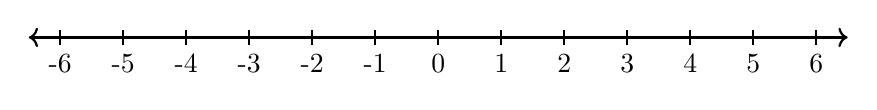
\begin{tikzpicture}[scale=0.8]
    \draw[<->, thick] (-6.5,0) -- (6.5,0);
    \foreach \x in {-6,-5,-4,-3,-2,-1,0,1,2,3,4,5,6}
    {
        \draw[thick] (\x,0.12) -- (\x,-0.12);
        \node[below] at (\x,-0.12) {\x};
    }
\end{tikzpicture}
\end{center}
}

\newcommand{\openpoint}[1]{
\draw[thick, fill=white] (#1,0) circle (0.13);
}

\newcommand{\closedpoint}[1]{
\draw[thick, fill=black] (#1,0) circle (0.13);
}

\begin{document}
\handwriting

\begin{center}
    \Large\textbf{\color{primaryblue}Module 1 Lesson 5\\Linear Inequalities} \\
    \vspace{0.2cm}
    \hrule
\end{center}

\section*{Objectives}

\begin{friendlyrule}{In this lesson, we will learn how to}
\begin{itemize}
    \item apply the addition and multiplication principles for inequalities;
    \item solve linear and double inequalities;
    \item express solutions in interval notation and on a number line;
    \item apply inequalities to real-world problems.
\end{itemize}
\end{friendlyrule}

\section*{1. Principles for Solving Inequalities}

An \funhl{inequality} is a mathematical sentence containing $<$, $>$, $\le$, or $\ge$. The solution is all values of the variable that make the inequality true.

\begin{friendlyrule}{Addition Principle}
For any real numbers $a$, $b$, $c$: if $a<b$ is true, then $a+c<b+c$ is true.
\end{friendlyrule}

\begin{friendlyrule}{Multiplication Principle}
\begin{itemize}
    \item[(a)] If $a<b$ and $c>0$, then $ac<bc$.
    \item[(b)] If $a<b$ and $c<0$, then $ac>bc$.
\end{itemize}
\end{friendlyrule}

\begin{friendlyrule}{Important Note}
When both sides of an inequality are multiplied (or divided) by a \textbf{negative} number, the inequality sign must be \textbf{reversed}.
\end{friendlyrule}

\begin{friendlyex}
Solve each inequality. Express the solution in interval notation, and graph the solution.

\begin{itemize}
    \item[(a)] $2x-1>x+5$
    \item[(b)] $3-2x<x+9$
    \item[(c)] $-\dfrac12 x\ge 2+\dfrac23 x$
\end{itemize}
\end{friendlyex}

\blanknumberline
\blanknumberline
\blanknumberline

\begin{solutionbox}
\textbf{(a)}

\[
2x-1>x+5.
\]

\[
2x-x>5+1.
\]

\[
x>6.
\]

Interval notation: $(6,\infty)$.

\[
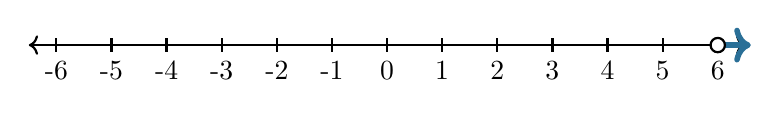
\begin{tikzpicture}[scale=0.7]
    \draw[<->, thick] (-6.5,0) -- (6.5,0);
    \foreach \x in {-6,-5,-4,-3,-2,-1,0,1,2,3,4,5,6}
    {
        \draw[thick] (\x,0.12) -- (\x,-0.12);
        \node[below] at (\x,-0.12) {\x};
    }
    \draw[line width=2pt, primaryblue, ->] (6,0) -- (6.6,0);
    \openpoint{6}
\end{tikzpicture}
\]

\textbf{(b)}

\[
3-2x<x+9.
\]

\[
3-9<x+2x.
\]

\[
-6<3x.
\]

\[
x>-2.
\]

Interval notation: $(-2,\infty)$.

\[
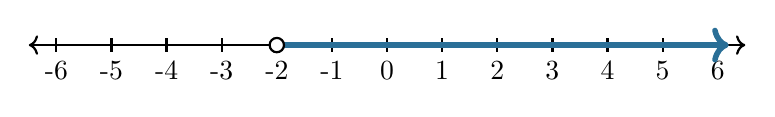
\begin{tikzpicture}[scale=0.7]
    \draw[<->, thick] (-6.5,0) -- (6.5,0);
    \foreach \x in {-6,-5,-4,-3,-2,-1,0,1,2,3,4,5,6}
    {
        \draw[thick] (\x,0.12) -- (\x,-0.12);
        \node[below] at (\x,-0.12) {\x};
    }
    \draw[line width=2pt, primaryblue, ->] (-2,0) -- (6.2,0);
    \openpoint{-2}
\end{tikzpicture}
\]

\textbf{(c)} Multiply both sides by $6$ to clear fractions:

\[
6\left(-\frac12 x\right)\ge 6(2)+6\left(\frac23 x\right).
\]

\[
-3x\ge 12+4x.
\]

\[
-7x\ge 12.
\]

Dividing by $-7$ \textbf{reverses} the inequality:

\[
x\le -\frac{12}{7}.
\]

Interval notation: $\left(-\infty,-\dfrac{12}{7}\right]$.

\[
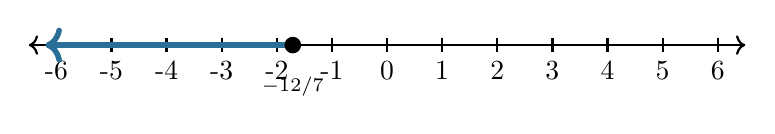
\begin{tikzpicture}[scale=0.7]
    \draw[<->, thick] (-6.5,0) -- (6.5,0);
    \foreach \x in {-6,-5,-4,-3,-2,-1,0,1,2,3,4,5,6}
    {
        \draw[thick] (\x,0.12) -- (\x,-0.12);
        \node[below] at (\x,-0.12) {\x};
    }
    \draw[line width=2pt, primaryblue, <-] (-6.2,0) -- (-1.71,0);
    \closedpoint{-1.71}
    \node[below] at (-1.71,-0.4) {\scriptsize $-12/7$};
\end{tikzpicture}
\]
\end{solutionbox}

  

\section*{2. Double Inequalities}

\begin{friendlyex}
Solve each double inequality. Express the solution in interval notation and graph the solution.

\begin{itemize}
    \item[(a)] $3<5+4x<6$
    \item[(b)] $2x-3\le 4x+3<2x+5$
\end{itemize}
\end{friendlyex}

\blanknumberline
\blanknumberline

\begin{solutionbox}
\textbf{(a)} Subtract $5$ from all three parts:

\[
-2<4x<1.
\]

Divide by $4$:

\[
-\frac12<x<\frac14.
\]

Interval notation: $\left(-\dfrac12,\dfrac14\right)$.

\[
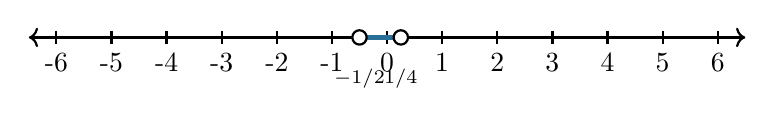
\begin{tikzpicture}[scale=0.7]
    \draw[<->, thick] (-6.5,0) -- (6.5,0);
    \foreach \x in {-6,-5,-4,-3,-2,-1,0,1,2,3,4,5,6}
    {
        \draw[thick] (\x,0.12) -- (\x,-0.12);
        \node[below] at (\x,-0.12) {\x};
    }
    \draw[line width=2pt, primaryblue] (-0.5,0) -- (0.25,0);
    \openpoint{-0.5} \openpoint{0.25}
    \node[below] at (-0.5,-0.4) {\scriptsize $-1/2$};
    \node[below] at (0.25,-0.4) {\scriptsize $1/4$};
\end{tikzpicture}
\]

\textbf{(b)} Split into two inequalities.

Left: $2x-3\le 4x+3\ \Longrightarrow\ -6\le 2x\ \Longrightarrow\ x\ge -3$.

Right: $4x+3<2x+5\ \Longrightarrow\ 2x<2\ \Longrightarrow\ x<1$.

Combining:

\[
-3\le x<1.
\]

Interval notation: $[-3,1)$.

\[
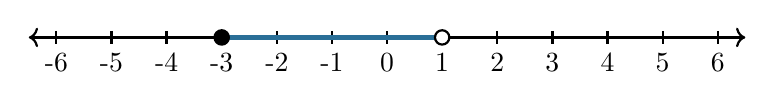
\begin{tikzpicture}[scale=0.7]
    \draw[<->, thick] (-6.5,0) -- (6.5,0);
    \foreach \x in {-6,-5,-4,-3,-2,-1,0,1,2,3,4,5,6}
    {
        \draw[thick] (\x,0.12) -- (\x,-0.12);
        \node[below] at (\x,-0.12) {\x};
    }
    \draw[line width=2pt, primaryblue] (-3,0) -- (1,0);
    \closedpoint{-3} \openpoint{1}
\end{tikzpicture}
\]
\end{solutionbox}

  

\section*{3. Verbal Problems and Applications}

\begin{friendlyex}
\begin{itemize}
    \item[(a)] If $55$ more than $x$ is bigger than $-124$, determine all possible values of $x$.
    \item[(b)] Ethan has $\$90$ to spend on juice boxes. Each juice box costs $\$2.51$. What is the maximum number of juice boxes he can buy?
    \item[(c)] Saanvi can be paid in one of two ways for painting a house: Plan A pays $\$200$ plus $\$12$ per hour; Plan B pays $\$20$ per hour. If a job takes $n$ hours, for what values of $n$ is Plan A better financially?
\end{itemize}
\end{friendlyex}

 

\begin{solutionbox}
\textbf{(a)}

\[
x+55>-124.
\]

\[
x>-179.
\]

Interval notation: $(-179,\infty)$.

\textbf{(b)} We need

\[
2.51n\le 90.
\]

\[
n\le \frac{90}{2.51}\approx 35.86.
\]

Since $n$ must be a whole number, the maximum is $n=35$ juice boxes.

\textbf{(c)} Plan A pays $200+12n$; Plan B pays $20n$. Plan A is better when

\[
200+12n>20n.
\]

\[
200>8n.
\]

\[
n<25.
\]

Plan A is the better financial choice when the job takes \textbf{fewer than $25$ hours}.
\end{solutionbox}

  

\section*{Summary}

\begin{friendlyrule}{Key Ideas}
\begin{itemize}
    \item Adding or subtracting the same number from both sides of an inequality never changes the direction of the inequality.
    \item Multiplying or dividing both sides by a \textbf{negative} number \textbf{reverses} the inequality sign.
    \item Use an open circle for $<$ or $>$, and a closed circle for $\le$ or $\ge$.
    \item Double inequalities can be solved all at once (if the variable appears the same way in all parts) or split into two separate inequalities and combined.
    \item Solutions are typically expressed using interval notation and graphed on a number line.
\end{itemize}
\end{friendlyrule}

\end{document}
